
\subsubsection*{Problem definition}

The aim of this example is to simulate the stationary groundwater flow in an isotropic and heterogeneous porous medium. In order to consider the heterogeneous of permeability, a 2~D numerical model was built. The heterogeneous distribution of permeability is showed in \ref{KDis}.
\begin{figure}[htbp]
\centering
\includegraphics[width=0.8\textwidth]{H_GW/figures/KDis.eps}
\caption{Calculation model(2~D): hetergeneous permeability distribution}
\label{KDis}
\end{figure}

\textsl{Assumptions}

\begin{tabbing}
\=xxxxxxxxxxxxx  \=xxxxxxxxxxxxxxxxxxxxxxx \kill
\> Aquifer: \> isotropic, heterogeneous, saturated, stationary flow
\end{tabbing}

\subsubsection*{Model set-up of the 2~D numerical model}

For the 2-dimensional simulation, the cube consisting of a porous medium is simplified as a square with an area of 10000~m$^2$. The calculation model includes 10000 quad elements and 10201 nodes. At the left boundary  a constant head of 10~m and the right boundary  a constant head of 9~m are specified in order to create a pressure gradient. 

\subsubsection*{Results}

In figure \ref{HeadDis} the horizontal and vertical head distributions of a groundwater flow in a heterogeneous medium are depicted responsing to the distribution of the permeability. 

\begin{figure}[htbp]
\centering
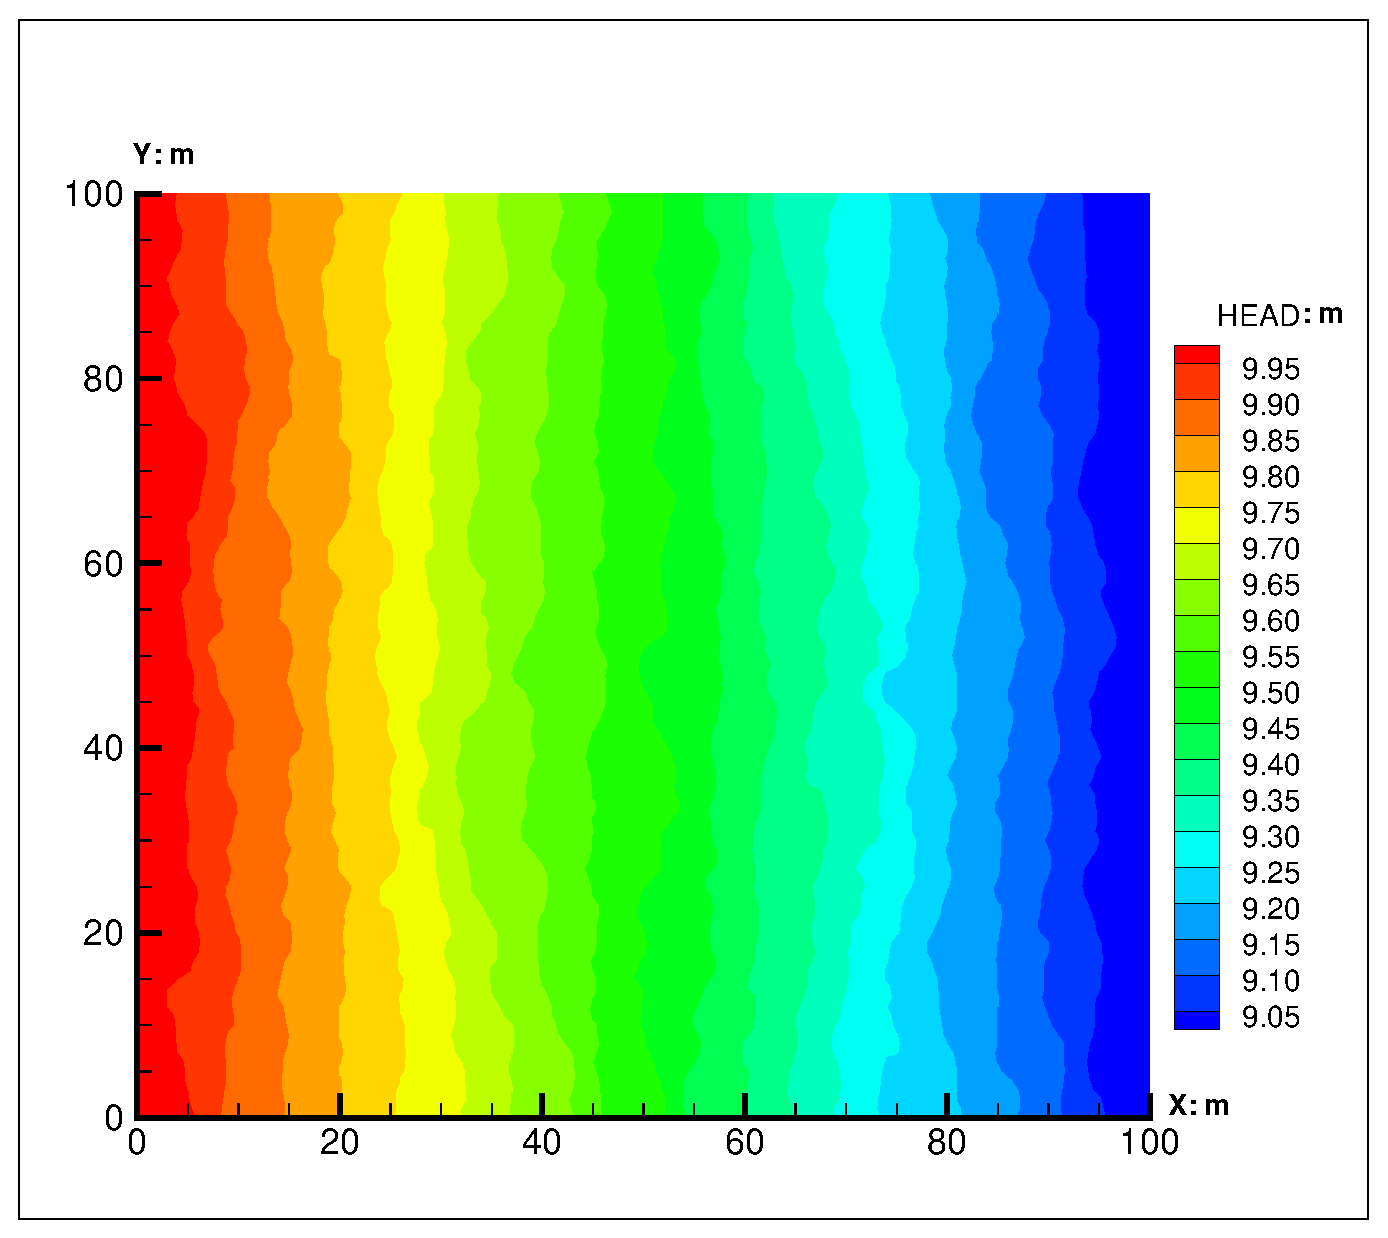
\includegraphics[width=0.8\textwidth]{H_GW/figures/HeadDis.eps}
\caption{Head distribution responsed to isotropic and heterogeneous medium}
\label{HeadDis}
\end{figure}

\begin{tabular}{|l|l|l|}
\hline
Benchmark & Problem type	& Path in benchmark deposit \\
\hline	
2D1P-GWFlow	& H	& benchmarks $\backslash$H$\backslash$HetGWFlow \\
\hline	
\end{tabular}